\chapter{Conceito do Sistema}
\label{chap:concep}

A percepção do ELIR pode ser definida como um sistema de sensoriamento integrado com unidades de processamento para disponibilizar os dados com maior confiabilidade e  transparência ao operador final. O sistema foi projetado de forma a possuir três subsistemas principais: segurança, georreferenciamento e detecção. A descrição de cada um dos subsistemas e suas funcionalidades serão mostradas nas próximas sessões.


%--------- NEW SECTION ----------------------
%\section{Estudo do estado da arte}
%\label{sec:sota}
%flkjasdlkfjasdlkfjs

%--------- NEW SECTION ----------------------
\section{Descrição do sistema}
\label{sec:desc}
O sistema de Percepção foi projeto de forma a atender as necessidades do processo de inspeção de uma linha de transmissão. 

Buscando identificar os trechos de falha, o sistema dispõe de uma câmera térmica para realizar a identificação de pontos quentes na linha e em seus obstáculos permitindo um diagnóstico prévio da inspeção. O sistema também possui sub-sistemas de georreferenciamento e navegação do robô. Estes ajudam a identificar facilmente os locais de falhas na linha na qual a equipe de manutenção deve operar e também fornecem informações de posicionamento e orientação do robô.

Para manter a integridade física do robô, o sub-sistema de segurança possui sensores de proximidade em todas as suas garras para identificar se as mesmas se encontram na linha de transmissão ou não. Além disso, é monitorada a temperatura na housing eletrônica, corrente nos motores e consumo energético do sistema. 


Todos os dados obtidos durante a missão e as informações de segurança do robô são apresentados através de uma interface gráfica. Nesta interface o operador pode acompanhar em tempo real as inspeções realizadas através da câmera térmica, a informação dos atuadores, dados de integridade do robô e todas as ocorrências. 

\subsection{Especificação técnica}
\label{ssec:espt}

\begin{itemize}
\item O sistema foi projetado para trabalhar com alimentação de 14V proveniente de baterias LiPo.
\item A máxima temperatura de trabalho é 50 graus Celsius.
\item O sistema consegue detectar objetos através do sonar em uma faixa de servidão de 6.45 metros.
\item A obtenção de frames da câmera IR acontece na taxa de 1 frame/seg.
\item Em condições de sobretemperatura e sobrecorrente o sistema entra em modo de emergência.
\item O sistema não é protegido contra ingresso de água
\end{itemize} 




\subsection{Arquitetura geral do sistema}
\label{ssec:arqg}
A Percepção é o sistema de sensoriamento do robô e pode ser entendida como a forma que ele compreende o que esta ao seu redor. No projeto do robô ELIR o sistema de percepção engloba a aquisição e a interpretação dos dados de todos os sensores envolvidos.

Na arquitetura geral deste sistema, mostrado na Fig. \ref{arqgeral}, estão representados as três camadas principais: Sensing, Interface e ROS Enviroment.

\begin{figure}[!ht]
\centering
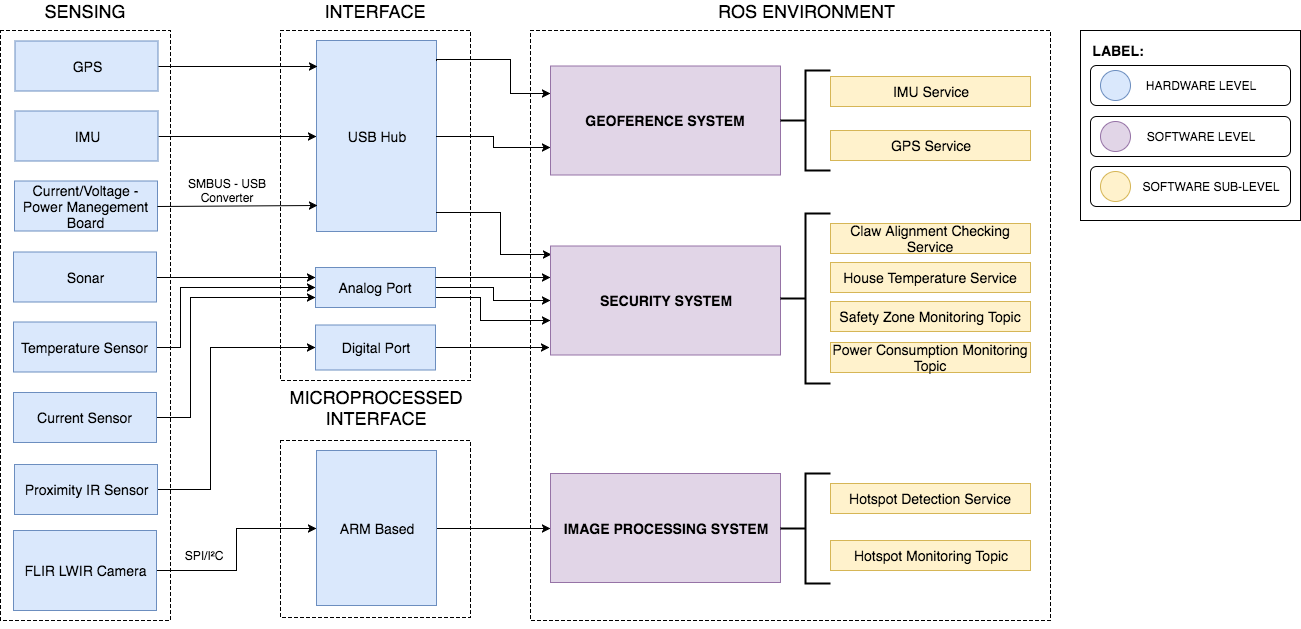
\includegraphics[width=15cm]{Figures/ArquiteturaPerceptionv2.png}
\caption{Arquitetura Geral da Perception}\label{arqgeral}
\end{figure}

 A etapa de Sensing é composta por todos os processos de aquisição de dados de todos os sensores envolvidos no projeto. A camada de interface compreende a disponibilização destes dados para o ambiente de trabalho ROS. Essas duas etapas são camadas de hardware. Por último, terá a camada de software, a qual será feita no ROS Enviroment, e que irá englobar todo o sistema de compreensão e interpretação dos dados provenientes do sistema de interfaceamento do robô.
 
\subsection{Arquitetura de software}

A arquitetura de software foi projetada em três camadas a fim de facilitar o desenvolvimento do sistema e simplificar o entendimento do mesmo. As camadas de software são:

\begin{itemize}
\item User Interface Layer
\item Business Layer
\item Driver Layer
\end{itemize} 
As camadas e seus componentes podem ser vistos na Fig.\ref{arqsoft}.
\begin{figure}[H]
\centering
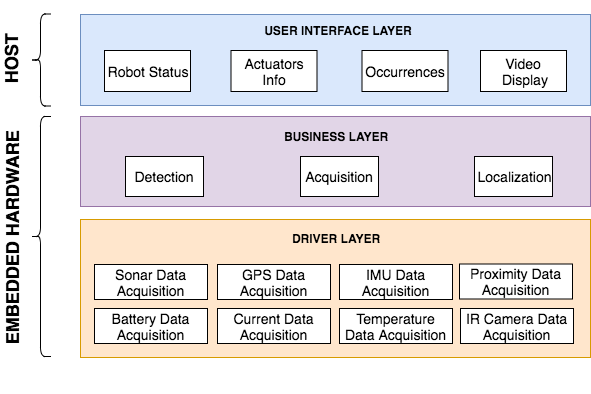
\includegraphics[width=15cm]{Figures/ArquiteturadeSoftware.png}
\caption{Arquitetura Geral da Perception}\label{arqsoft}
\end{figure}

\subsubsection{Driver Layer}
A camada de Driver Layer está diretamente relacionada a funcionalidade de aquisição de dados. Ela composta por partes físicas representadas pelos sensores e seus respectivos drivers de comunicação. Desta forma, as subcamadas são nomeadas com o processo de aqusição de dados de cada sensor envolvido no projeto.

As subcamadas \textit{Current Data Acquisition}, \textit{Temperatura Data Acquisition}, \textit{Proximity Data Acquisition} e \textit{Sonar Data Acquisition} são responsáveis por adquirir as informações analógicas de seus sensores e transformá-los em dados da grandeza física a ser medida. Todas estas subcamadas utilizam a placa de interfaceamento Phidgets para o estabeler de comunicação entre a NUC e os sensores.

As subcamadas \textit{IMU Data Acquisition} e \textit{GPS Data Acquisition} são responsáveis pelo recebimento de dados da IMU e do GPS seguindo o protocolo de comunicação do fabricante. 

A subcamada de \textit{IR Camera Data Acquisition} é responsável pela aquisição de dados da câmera térmica. 
Por último, a subcamada de \textit{Battery Data Acquisition} é responsável pelo estabelecimento da comunicação e coleta de informações com a placa multiplexadora de bateria utilizando protocolo I2C.

\subsubsection{Business Layer}

A camada de business layer é responsável por implementar a regra de negócio do sistema. A sub-camada management é quem realiza o processo de gerenciamento e controle das funcionalidades e por isso é representada com nível hierárquico maior do que as demais sub-camadas. As funcionalidades do sistema são representadas como sub-camadas da business layer pois ela são responsáveis pelo processamento e coordenação de dados adquiridos pela camada de aquisição. 


\subsubsection{User Interface Layer}

A camada de User Interface foi projetada para facilitar a interação com o usuário final. Ela tem o objetivo de disponibilizar de forma simplificada os dados mais relevantes do robô. Nesta camada existem três subcamadas: Robot Status Display, Actuators Display e Video Display. A subcamada Robot Status Display disponibiliza os dados de integridade do robô como temperatura, corrente, tensão, nível de bateria, entre outras informações. A subcamada de Actuators Display, disponibiliza o dados de todos os motores do robô, como carga, temperatura, status e corrente, desta forma o usuário pode acompanhar o desenvolvimento de todas as suas atividades. Por último, a subcamada de Video Display mostra em tempo real o monitoramento realizado pela câmera infravermelho e estéreo possibilitando o usuário de ver os componentes da linha que estão com temperatura elevada e até mesmo identificar pontos quentes, assim como verificar a imagem no plano RGB.

A interface irá se resumir em duas telas: A tela principal com um layout de dashboard, e outra que será as informações dos atuadores. O dashboard será um painel de monitoramento, no qual haverá as informações mais importantes da missão, como pode ser visto na Fig. \ref{UI} no apêndice D. Essa tela, além de monstrar as informações, irá pode dar o comando de início e parada da missão a partir dos botões "Start" e "Stop". A tela dos atuadores irá mostrar de forma organizada, as informações que foram mencionadas, além da corrente total de cada HUB de motores. Pode-se observar a tela de atuadores na Fig. \ref{UI2} no apêndice C.

\label{ssec:arqs}

%--------- NEW SECTION ----------------------
%\section{Desdobramento da função qualidade}
%\label{sec:qfd}
%asdfsdafsf

%\subsection{Requisitos técnicos}
%\label{ssec:reqt}
%asdfsadfdsf

